%----------------Cap_03----------------%

\chapter{COMANDOS BÁSICOS EM LATEX}

Este capítulo é dedicado a apresentar ao mestrando alguns comandos básicos em LaTeX e que possivelmente serão utilizados para a estrita de sua dissertação. Dentre os inúmeros manuais de LaTeX em PDF encontrados em sites da \textit{internet}, selecionamos os seguintes como fundamento teórico para a confecção deste tópico:
\begin{itemize}
	\item \textbf{Edición de textos científicos LaTeX} - Um dos mais completos manuais para uso do LaTeX, este manual apresenta inúmeros recursos para a personalização do documento em LaTeX. O manual em versão atualizada está disponível no endereço \url{https://tecdigital.tec.ac.cr/revistamatematica/Libros/LATEX/LaTeX_2013.pdf} \cite{latex-walter};
	\item \textbf{Tutorial de uso do LaTex para escrita científica} - Manual de LaTeX orientado para a escrita de trabalhos científicos com o uso do editor de textos TexMaker, disponível em \url{http://sbi.iqsc.usp.br/files/Manual-SBI_LATEX_2013-.pdf} \cite{latex-usp};
	\item \textbf{Uma não tão pequena
introdução ao LATEX 2$\varepsilon$} - Um consiso manual de LaTex que estruturado de acordo com os principais comandos da linguagem. Este manual pode ser encontrado para \textit{download} no endereço \url{ftp://ctan.tug.org/tex-archive/info/lshort/portuguese/pt-lshort-a5.pdf} \cite{oetiker}.
\end{itemize}

Além destes, ao longo do texto, outros manuais com temáticas específicas podem ser sugeridos. Uma fonte de pesquisa sobre a linguagem LaTeX propriamente dita pode ser encontrada no site do Projeto LaTeX (em tradução livre) onde o leitor interessado pode conhecer como surgiu a linguagem, a filosofia por trás do projeto e ainda encontrar documentação LaTeX \cite{LaTeX-Project}.

Outros manuais podem ser encontrados na \textit{internet}. Para quem tem interesse em um aprendizado mais ``dinâmico'', existem cursos completos de introdução ao LaTeX em em formato de video-tutoriais em sites como \textit{youtube}. 

\section{Estrutura básica do documento em latex}

A escrita de um documento em LaTeX resume-se a algumas ações: Assim que se abre um editor de LaTeX e cria-se um novo documento em branco, deve-se criar um \textbf{preâmbulo} onde se especifica a \textit{classe} e os \textit{pacotes} que serão utilizados para a configurção geral do documento. Em seguida, edita-se o corpo do documento em um local específico. Por fim, basta \textit{compilar} o código-fonte para visualizar o resultado na tela do computador em formato PDF (ou DVI).

A figura abaixo exemplifica o procedimento descrito acima na tela do editor TexMaker, para a escrita de um problema de matemática básica encontrado em \citeonline[p.~174]{Mat_ensmed_1}:
	\begin{figure}[H]
	\centering
	\caption{Exemplo de estrutura em LaTeX}
	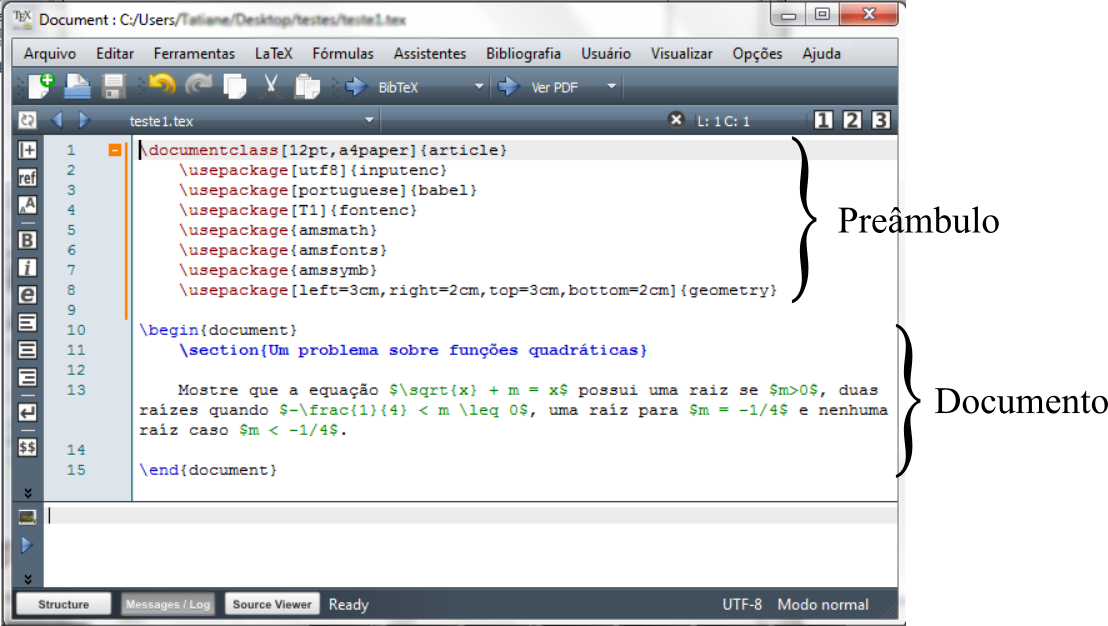
\includegraphics[scale=0.5]
	{img/fig01.png}\label{fig01}\\
	FONTE: Autor (2015)
	\end{figure}
	O \textbf{preâmbulo} contém o comando
\begin{verbatim}
\documentclass[12pt,a4paper]{article}
\end{verbatim}
com o qual se especifica, entre chaves \verb!{}!, a classe de documento. No exemplo dado, utilizou-se a classe \textit{article} adequada para confecção de documentos em formato de artigo. As opções da classe são inseridas entre colchetes \verb![]!. No exemplo, as opções usadas são o tamanho da fonte (12pt) e o formato da folha (A4). Outras classes comuns são ``book'' ou ``report'' \cite{latex-walter}. Neste modelo de dissertação, utiliza-se a classe ``abntex2'', derivada da classe ``memoir''.

No preâmbulo, ainda encontram-se os pacotes, indicados pelos comandos do tipo
\begin{verbatim}
\usepackage[opções]{nome-do-pacote}
\end{verbatim}

No exemplo da figura, o comando \verb!\usepackage[utf8]{inputenc}! habilita o uso de acentos diretamente do teclado, enquanto o comando \verb!\usepackage[portuguese]{babel}! permite que o editor reconheça palavras no idioma indicado nas opções, no caso português. Os pacotes \verb!amsmath!, \verb!amsfonts! e \verb!amssymb! habilitam o uso de símbolos e caracteres matemáticos. O comando
\begin{verbatim}
\usepackage[left=3cm,right=2cm,top=3cm,bottom=2cm]{geometry}
\end{verbatim}
configura as margens do documento, como pode ser visto nas opções entre colchetes.

Todo o documento deve ser escrito entre os comandos:
\begin{verbatim}
	\begin{document}

	\end{document}
\end{verbatim}

Estes comandos informam programa editor LaTeX onde começa e onde termina o documento. Além destes comandos, nada será compilado no documento final e entre eles, é possível dividir o documento em capítulos, seções e subseções, escrever fórmulas matemáticas, inserir figuras, etc, conforme será visto nos tópicos seguintes. Para finalizar esta seção, a figura abaixo ilustra o resultado em PDF dos comandos mostrados na Figura \ref{fig01}.
	\begin{figure}[H]
	\centering
	\caption{Visão em PDF de uma documento escrito em LaTeX}
	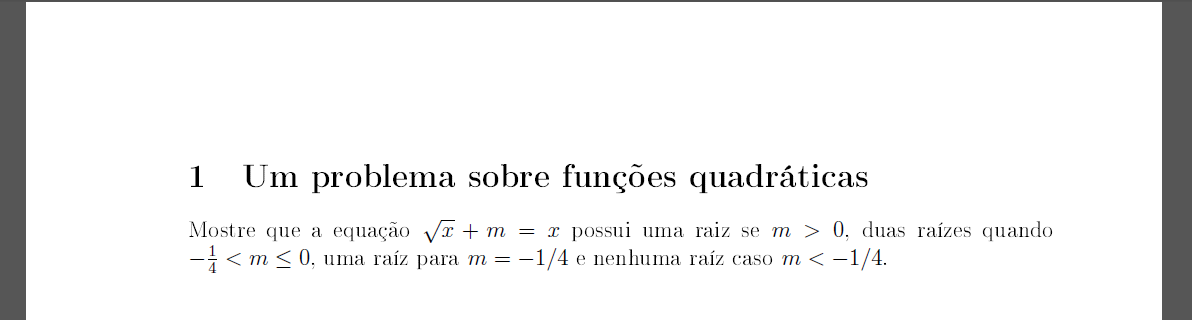
\includegraphics[scale=0.4]
	{img/fig02.png}\label{fig02}\\
	FONTE: Autor (2015)
	\end{figure}
	
\section{Formas de exibição de texto}

\subsection{Caracteres reservados}

Na linguagem LaTeX, alguns caracteres são \textbf{reservados} para que cumpram uma função específica dentro do programa. Assim, não é possível digitá-los simplesmente teclando sobre eles como se faz com uma letra qualquer. Quando se deseja digitar algum destes caracteres reservados, é preciso usar um comando específico. 

A Figura \ref{fig01} pode exemplificar esta situação.  Nela, percebe-se que quase todos os comando em LaTeX começam por uma ``barra invertida'' (\verb!\!). Comparando as Figuras \ref{fig01} e \ref{fig02}, percebe-se ainda que todas as expressões matemáticas no documento PDF correspondem a uma expressão escrita no código-fonte da Figura \ref{fig01} entre \verb!$$!. De fato, esta é uma das formas de escrever expressões em modo matemático. 

As tabelas abaixo mostram alguns destes caracteres. A primeira tabela indica a função do caractere dentro do programa LaTeX enquanto a segunda mostra que comando usar quando se quer que o caractere seja visualizado no documento final.
	\begin{table}
	\begin{center}
	\caption{Exemplos de caracteres reservados}
	\begin{tabular}{ c  c }
	\hline
	Caractere & Função no LaTeX:\\
	\hline
	\hline
	\verb!\! & caractere inicial de comando\\
	\verb!$$! & inicia e termina o modo matemático\\
	\verb!{ }! & inicia e termina um bloco de código\\
	\verb!&! & tabulador (em tabelas e matrizes)\\
	\verb!_! & escrever subíndice\\
	\verb!^! & escrever expoentes\\
	\verb!%! & escrever comentários\\
	\hline
	\end{tabular}\\ \vspace{0.25cm}
	FONTE: Autor (2015)
	\end{center}
	\end{table}

	
	\begin{table}
	\begin{center}
	\caption{Comandos para impressão de caracteres reservados}
	\begin{tabular}{ c  c }
	\hline
	Caractere & Comando para impressão:\\
	\hline
	\hline
	\$ & \verb!\$!\\
	\{ , \} & \verb!\{ , \}! \\
	\& & \verb!\&! \\
	\_ & \verb!\_! \\
	%\^ & \verb!\^! \\
	\% & \verb!\%! \\
	\hline
	\end{tabular}\\ \vspace{0.25cm}
	FONTE: Autor (2015)
	\end{center}
	\end{table}
	
	
\subsection{Mudando o estilo e o tamanho das fontes}	

O LaTeX permite ao usuário uma variedade de formas de exibição do texto. Os comandos abax exemplificam comomudar o estilo de fonte usada no texto:
\begin{itemize}
	\item O comando \verb!\textbf{texto em negrito}! produz \textbf{texto em negrito};
	\item O comando \verb!\textit{texto em itálico}! produz \textit{texto em itálico};
	\item O comando \verb!\textrm{texto em romano}! produz \textrm{texto em romano};
	\item O comando \verb!\textsf{texto em sans sefif}! produz \textbf{texto em sans serif};
	\item O comando \verb!\textsc{texto em caixa alta}! produz \textbf{texto em caixa alta};
\end{itemize}

O tamanho da letra também pode ser modificado:
\begin{itemize}
	\item O comando \verb!{\tiny um texto pequeníssimo}! produz {\tiny um texto pequeno};
	\item O comando \verb!{\scriptsize um texto muito pequeno}! produz {\scriptsize um texto muito pequeno};
	\item O comando \verb!{\footnotesize um texto pequeno}! produz {\footnotesize um texto pequeno};
	\item O comando \verb!{\large um texto grande}! produz {\large um texto grande};
	\item O comando \verb!{\Large um texto maior}! produz {\Large um texto maior};
	\item O comando \verb!{\LARGE um texto muito maior}! produz {\LARGE um texto muito maior};
	\item O comando \verb!{\huge um texto enorme}! produz {\huge um texto enorme};
	\item O comando \verb!{\Huge um texto ainda maior}! produz {\Huge um texto ainda maior}.
\end{itemize}

Ainda é possível combinar os comandos de estilo e tamanho de letra. Por exemplo, para escrever um texto em negrito com tamanho grande, basta escrever
\begin{verbatim}
{\Large \textbf{texto grande e em negrito}}
\end{verbatim}
o resultado será:
\begin{center}
{\Large \textbf{texto grande e em negrito}}.
\end{center}

\section{Criando listas}

A criação de listas sejam elas estruturadas em tópicos ou numeradas  também é facilitada utilizando a escrita em LaTeX. Em ambos os casos, deve-se utilizar um ``ambiente'' específico. Um ambiente é um bloco de comandos LaTeX que recebe uma formatação especial. Todo ambiente deve começar pelo comando \verb!\begin{nome-do-ambiente}! e terminar com o comando \verb!\end{nome-do-ambiente}!.

No que segue, são mostrados os ambientes \texttt{itemize} para criação de listas estruturadas em tópicos e o ambiente \texttt{enumerate} para listas numeradas.

\subsection{Ambiente itemize}

Os comandos abaixo exemplificam e caracterizam o ambiente \texttt{itemize}
	\begin{figure}[H]
	\centering
	\caption{Lista usando o ambiente \texttt{itemize} em latex}
	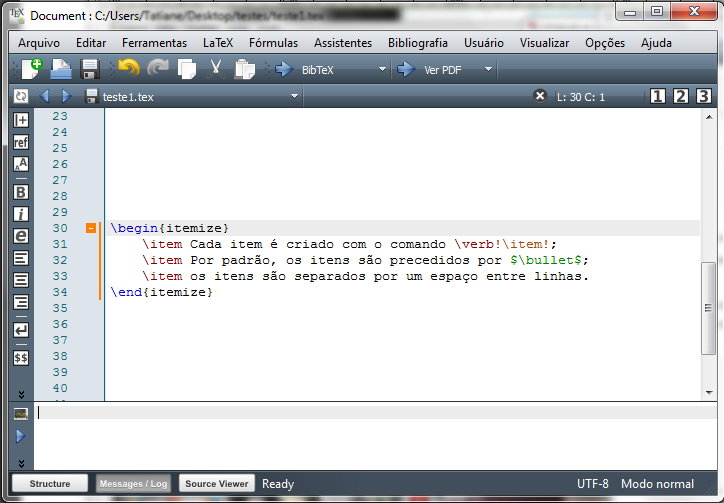
\includegraphics[scale=0.5]
	{img/fig03.png}\label{fig03}\\
	FONTE: Autor (2015)
	\end{figure}

O resultado é mostrado na figura abaixo:
	\begin{figure}[H]
	\centering
	\caption{Lista usando o ambiente \texttt{itemize}  - resultado em tela}
	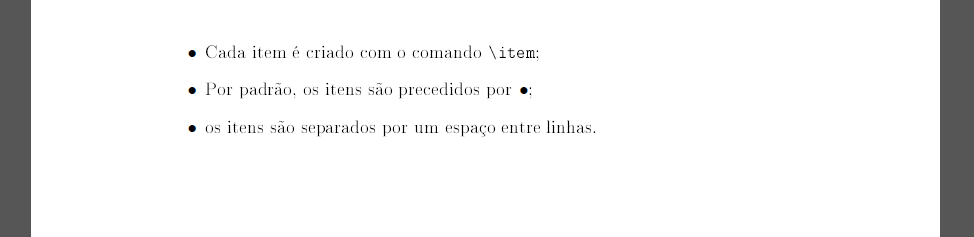
\includegraphics[scale=0.4]
	{img/fig04.png}\label{fig04}\\
	FONTE: Autor (2015)
	\end{figure}
	

\subsection{Ambiente enumerate}

O exemplo a seguir ilustra o uso do ambiente \texttt{enumerate}. Observe que é possível adicionar subníveis dentro de um mesmo ambiente ou ainda mesclar dois ambientes de listas:
	\begin{figure}[H]
	\centering
	\caption{Lista usando o ambiente \texttt{enumerate} em latex}
	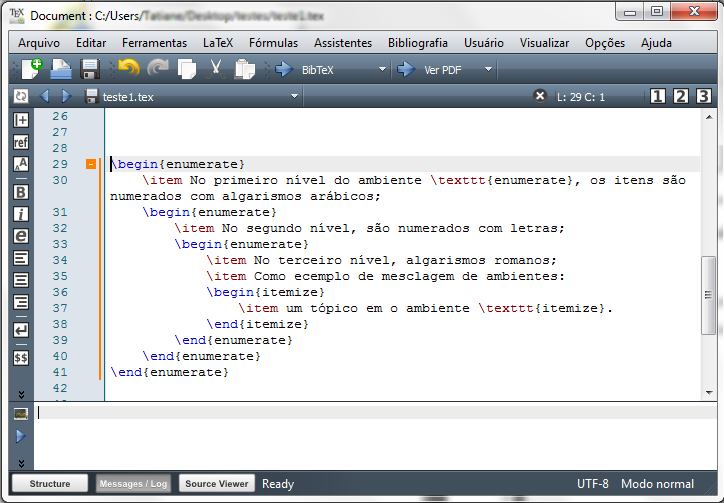
\includegraphics[scale=0.5]
	{img/fig05.png}\label{fig05}\\
	FONTE: Autor (2015)
	\end{figure}

	\begin{figure}[H]
	\centering
	\caption{Lista usando o ambiente \texttt{enumerate} - resultado em tela}
	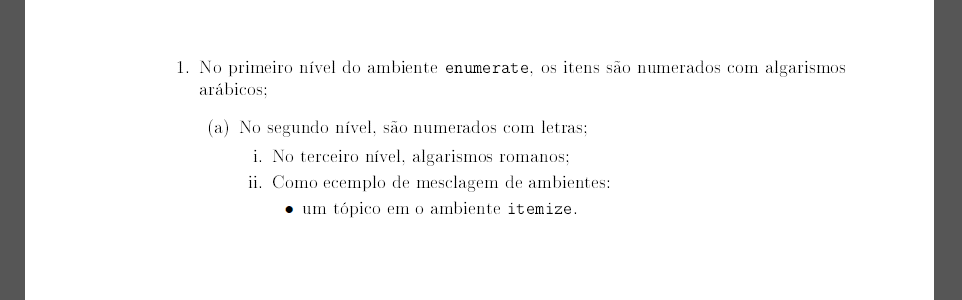
\includegraphics[scale=0.4]
	{img/fig06.png}\label{fig06}\\
	FONTE: Autor (2015)
	\end{figure}


\section{Escrevendo fórmulas matemáticas}

Em LaTeX, existem comandos específicos para escrever os mais diversos tipos de fórmulas e expressões matemáticas usando o \textbf{modo matemático}.

A forma mais simples de escrever uma expressão em modo matemático é usando os caracteres \verb!$!. Quando se deseja escrever uma expressão matemática dentro do parágrafo, basta iniciá-la e terminá-la com o símbolo \verb!$!. Por exemplo, a expressão $ax^2 + bx + c = 0$ é produzida digitando-se \verb!$ax^2 + bx + c = 0$!. Por outro lado, se se deseja deixar a expressão destacada do texto principal, ao invés de um caractere \verb!$!, utiliza-se dois caracteres \verb!$$! para iniciar o modo matemático e dois para terminar. Assim, por exemplo, a solução da equação do segundo grau acima é
$$
x=\frac{-b\pm\sqrt{b^2-4ac}}{2a}
$$
que no editor LaTeX foi produzida por meio dos comandos
\begin{verbatim}
$$
x=\frac{-b\pm\sqrt{b^2-4ac}}{2a}
$$
\end{verbatim}

Se o trabalho apresenta um grande número de equações e expressões,pode ser interessante, além de destacá-las do texto, numerá-las. Isso pode ser feito por meio do ambiente \texttt{equation}. Por exemplo, usando os comandos
\begin{verbatim}
\begin{equation}
	p(x) = a_nx^n + a_{n-1}x^{n-1} + \cdots + a_1x +  a_0
\end{equation}
\end{verbatim}
tem-se como resultado
\begin{equation}
	p(x) = a_nx^n + a_{n-1}x^{n-1} + \cdots + a_1x + a_0.
\end{equation}

A tabela abaixo mostra alguns dos comandos e símbolos mais utilizados em modo matemático:
\begin{table}[H]
\begin{center}
\caption{Alguns símbolos matemáticos}
\begin{tabular}{c c c c}
\hline
Caractere & Aplicação & Em LaTeX & Em tela\\
\hline
\hline
\verb!^! & expoente & \verb!a^2! & $a^2$\\
\verb!_! & subscrito & \verb!N_3! & $N_3$\\
\verb!\frac{}{}! & fração & \verb!\frac{1}{2}! & $\frac{1}{2}$\\
\verb!\sqrt{}! & raiz quadrada & \verb!\sqrt{x}! & $\sqrt{x}$\\
\verb!\alpha, \beta! & letras gregas & \verb!\alpha, \beta! & $\alpha, \beta$\\
\verb!\sin! & seno & \verb!\sin \alpha! & $\sin \alpha$\\
\verb!\sum! & somatório & \verb!\sum\limits_{i=1}^n a_i! & $\sum\limits_{i=1}^n a_i$\\
\hline
\end{tabular}\\ \vspace{0.25cm}
FONTE: Autor (2015)
\end{center}
\end{table}

Uma lista mais completa de símbolos e caracteres matemáticos pode ser encontrada em \citeonline{big-list} ou, para uma pesquisa mais rápida, em  \citeonline{small-list}.

Para finalizar este tópico, são apresentados exemplos de comandos LaTeX para produção de matrizes
\begin{verbatim}
$$
A=
\left[
\begin{array}{ccc}
1&3&-2\\
2&1&4\\
0&2&0
\end{array}
\right]
$$
\end{verbatim}
cujo resultado é
$$
A=
\left[
\begin{array}{ccc}
1&3&-2\\
2&1&4\\
0&2&0
\end{array}
\right]
$$
e para sistemas de equações
\begin{verbatim}
\begin{eqnarray*}
		\left\lbrace
		\begin{aligned}
		&a_{11}x_1+a_{12}x_2 + \ldots + a_{1n}x_n = b_1\\
		&a_{21}x_1+a_{22}x_2 + \ldots + a_{2n}x_n = b_2\\
		&\quad \vdots \quad \qquad \qquad \ddots  \quad \qquad \qquad \vdots\\
		&a_{m1}x_1+a_{m2}x_2 + \ldots + a_{mn}x_n = b_m
		\end{aligned}
		\right.
\end{eqnarray*}
\end{verbatim}
com resultado em tela:
\begin{eqnarray*}
		\left\lbrace
		\begin{aligned}
		&a_{11}x_1+a_{12}x_2 + \ldots + a_{1n}x_n = b_1\\
		&a_{21}x_1+a_{22}x_2 + \ldots + a_{2n}x_n = b_2\\
		&\quad \vdots \quad \qquad \qquad \ddots  \quad \qquad \qquad \vdots\\
		&a_{m1}x_1+a_{m2}x_2 + \ldots + a_{mn}x_n = b_m
		\end{aligned}
		\right.
\end{eqnarray*}

\subsection{Inserindo ilustrações}

A inserção de ilustrações em documentos LaTeX é bastante simples. Entretanto, é necessário que no preâmbulo esteja o comando
\begin{verbatim}
\usepackage{graphicx}
\end{verbatim}
É possível inserir figuras dos mais diversos formatos: .png, .jpg, .pdf, dentre outros. No caso deste modelo de dissertação e para o correto funcionamento dos comandos nos exemplos a seguir,também é preciso que todas as figuras a serem utilizadas no trabalho estejam salvas na pasta \verb!img! que foi baixada junto com o código-fonte do modelo.

\begin{figure}[H]
	\centering
	\caption{Exemplo de estrutura em LaTeX}
	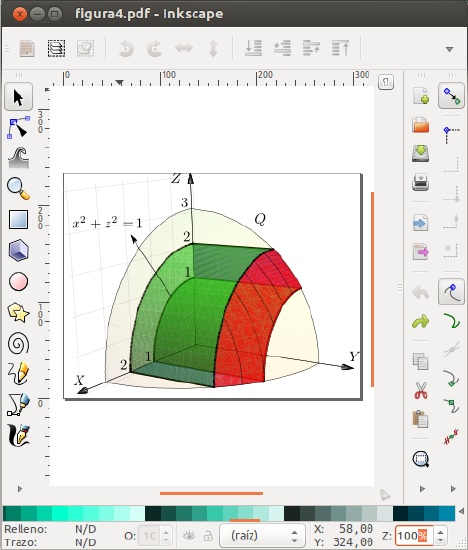
\includegraphics[scale=0.5]{img/fig07.png}\label{fig07}\\
	FONTE: \cite[p.~112]{latex-walter}
\end{figure}

Assim, por exemplo, para inserir a Figura \ref{fig07} deste modelo, foram utilizados os comandos:
\begin{verbatim}
	\begin{figure}[H]
	\centering
	\caption{Exemplo de estrutura em LaTeX}
	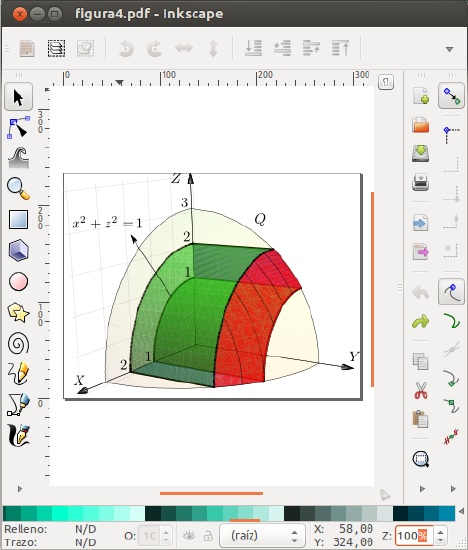
\includegraphics[scale=0.5]{img/fig07.png}\label{fig07}\\
	FONTE: \cite[p.~112]{latex-walter}
	\end{figure}
\end{verbatim}

Observe que tudo começa com o ambiente \texttt{figure}, iniciado pelo comando \verb!\begin{figure}! e terminado pelo comando \verb!\end{figure}!. A opção \verb![H]! fixa a figura no exato local onde o comando foi escrito, já que o LaTeX tem por padrão reposicionar as figuras (ou tabelas) para melhor distribuir o texto. A opção \verb!\centering! centraliza tudo o que vier após. 

O comando \verb!\caption{legenda-da-figura}! insere a legenda da figura. O comando \verb!\includegraphics[opçoes]{img/nome-da-figura.png}! insere a figura desejada. É possível redimensionar a figura alterando o número da opção \verb!scale = 0.5!. 


O comando \verb!\label{nome-do-objeto}! é uma ``etiqueta'' com a qual é possível identificar a figura (ou tabela, ou equação) e referenciá-la no texto. Para isso, basta escrever no documento o comando \verb! \ref{nome-do-objeto}!. Note que o \texttt{nome-do-objeto} na etiqueta \verb!\label{}! deve ser o mesmo no comando de referência \verb! \ref{}!.

Por fim, deve-se indicar a fonte da qual a figura foi retirada. Isso foi feito no exemplo acima por meio do comando \verb!\cite[]{}! cuja explicação é deixada para o próximo capítulo.


\subsection{Inserindo tabelas}

Para inserir tabelas em LaTeX, utiliza-se a sintaxe básica
\begin{verbatim}
\begin{tabular}{formato-das-colunas}
\hline
linha1 \\
\hline
linha2 \\
linha3 \\
\hline
\end{tabular}
\end{verbatim}

Em \texttt{formato-das-colunas}, deve-se especificar quantas colunas a tabelas irá conter, bem como o alinhamento. As opções possíveis para \texttt{formato-das-colunas} são
\begin{itemize}
	\item \texttt{l} - alinhamento à esquerda;
	\item \texttt{r} - alinhamento à direita;
	\item \texttt{c} - alinhamento centralizado.
\end{itemize}

Cada letra corresponderá a uma coluna.

O comando \verb!\hline! desenha uma linha horizontal de comprimento igual ao da tabela. Dois \verb!\hline! juntos produzem duas linhas horizontais com um pequeno espaço vertical entre elas.

Cada \texttt{linha} deve conter as entradas separadas pelo simbolo \verb!\&!  e terminadas por \verb!\\!. Este comando é responsável pela quebra de linha.

A fim de customizar a tabela criada, é aconselhável escrever os comandos da sintaxe mostrada acima dentro do ambiente \texttt{table}. Para centralizar a tabela, usa-se o ambiente \texttt{center}. Por exemplo, usando os comandos
\begin{verbatim}
	\begin{table}
	\begin{center}
	\caption{Exemplos de caracteres reservados}
	\begin{tabular}{ c  c }
	\hline
	Caractere & Função no LaTeX:\\
	\hline
	\hline
	\verb!\! & caractere inicial de comando\\
	\verb!$$! & inicia e termina o modo matemático\\
	\verb!{ }! & inicia e termina um bloco de código\\
	\verb!&! & tabulador (em tabelas e matrizes)\\
	\verb!_! & escrever subíndice\\
	\verb!^! & escrever expoentes\\
	\verb!%! & escrever comentários\\
	\hline
	\end{tabular}\\ \vspace{0.25cm}
	FONTE: Autor (2015)
	\end{center}
	\end{table}
\end{verbatim}
cujo resultado é mostrado na Tabela 1.


